% This is a combination of pandoc's default latex template:
% https://github.com/jgm/pandoc/blob/master/data/templates/default.latex

% and Dylan Mikesell's BSU thesis template:
% https://github.com/dylanmikesell/BSU_LaTeX_Thesis_Template/blob/master/src/BSUmain.tex

% and Dylan Mikesell's BSU style file:
% https://github.com/dylanmikesell/BSU_LaTeX_Thesis_Template/blob/master/src/BSUthesis.sty

% For BSU style requirements see:
% https://github.com/dylanmikesell/BSU_LaTeX_Thesis_Template/blob/master/src/BSU_checklist.pdf

% Pass options to packages loaded elsewhere
  \PassOptionsToPackage{dvipsnames,svgnames,x11names}{xcolor}

% Document class options
% Note: everything defined between \documentclass{} and \begin{document}
% is the "preamble"
\documentclass[
      12pt,
          twoside]{report}

% Loading packages and options

% Page geometry settings
\usepackage[
  left=1.5in,
  right=1in,
  top=1in,
  bottom=1in,
  letterpaper,
  includehead,
  includefoot,
  headheight=14.5pt
]{geometry}

% For colors
\usepackage[table]{xcolor} % Handles colors

% For better hyphenations
\usepackage{soulutf8}

% For landscape pages
\usepackage{pdflscape}

% For making corrections to functions
\usepackage{etoolbox}

% For strikeout and underline text
\usepackage[normalem]{ulem}

% Linespacing using setspace package
\usepackage{setspace}
\setstretch{2} % double space

% Math packages
\usepackage{amsmath,amssymb}

% Textcase for handling upper/lower case
\usepackage{textcase}

% Changepage package for changing layout in the middle of a document
\usepackage{changepage}

% For month year format
\usepackage{datetime}

% For chapter (and other) headings required by BSU
\usepackage{fancyhdr}

% Set captions styling
\usepackage[labelfont=bf,textfont=bf]{caption}
\captionsetup[figure]{
  font={
    stretch=0.6,
          small
      }
}

% For better float environments
\usepackage{float}

% For making tables and final reading approval page
\usepackage{tabularx}

% For setting (sub)section heading formatting and first paragraph spacing
\usepackage[explicit]{titlesec}

% For TOC style
\usepackage{titletoc}

% Font encoding
% Defaults to 8-bit T1 encoding with 256 glyphs
% https://ctan.org/pkg/encguide
% http://www.micropress-inc.com/fonts/encoding/t1.htm
\usepackage[T1]{fontenc}
\usepackage[utf8]{inputenc}
\usepackage{textcomp} % provide euro and other symbols

% Use upquote if available, for straight quotes in verbatim environments
\IfFileExists{upquote.sty}{\usepackage{upquote}}{}
\IfFileExists{microtype.sty}{% use microtype if available
  \usepackage[]{microtype}
  \UseMicrotypeSet[protrusion]{basicmath} % disable protrusion for tt fonts
}{}

% Font family setting
  % Default to adobe times new roman with math support
  \usepackage{mathptmx}

% Allow pandoc to inject code highlighting environments

% Tables settings
\usepackage{longtable,booktabs,array,threeparttable}
\usepackage{multirow}
\usepackage{calc} % for calculating minipage widths

% Correct order of tables after \paragraph or \subparagraph
\makeatletter
\patchcmd\longtable{\par}{\if@noskipsec\mbox{}\fi\par}{}{}
\makeatother

% Block quote shaded style
\usepackage{framed}
\AtBeginEnvironment{quote}{\par\singlespacing\small}
\let\oldquote=\quote
\let\endoldquote=\endquote
\colorlet{shadecolor}{gray!15}
\renewenvironment{quote}{\begin{shaded*}\begin{oldquote}}{\end{oldquote}\end{shaded*}}

% Allow footnotes in longtable head/foot
\IfFileExists{footnotehyper.sty}{\usepackage{footnotehyper}}{\usepackage{footnote}}
\makesavenoteenv{longtable}

% Graphics settings
\usepackage{graphicx}
\makeatletter
\def\maxwidth{\ifdim\Gin@nat@width>\linewidth\linewidth\else\Gin@nat@width\fi}
\def\maxheight{\ifdim\Gin@nat@height>\textheight\textheight\else\Gin@nat@height\fi}
\makeatother

% Scale images if necessary, so that they will not overflow the page
% margins by default, and it is still possible to overwrite the defaults
% using explicit options in \includegraphics[width, height, ...]{}
\setkeys{Gin}{width=\maxwidth,height=\maxheight,keepaspectratio}
% Set default figure placement to htbp
\makeatletter
\def\fps@figure{htbp}
\makeatother

% Prevent overfull lines
\setlength{\emergencystretch}{3em}
\providecommand{\tightlist}{\setlength{\itemsep}{0pt}\setlength{\parskip}{0pt}}

% Csl environment (required by pandoc)
  \newlength{\cslhangindent}
  \setlength{\cslhangindent}{1.5em}
  \newlength{\csllabelwidth}
  \setlength{\csllabelwidth}{3em}
  \newlength{\cslentryspacingunit} % times entry-spacing
  \setlength{\cslentryspacingunit}{\parskip}
  \newenvironment{CSLReferences}[2] % #1 hanging-ident, #2 entry spacing
   {% don't indent paragraphs
    \setlength{\parindent}{0pt}
    % turn on hanging indent if param 1 is 1
    \ifodd #1
    \let\oldpar\par
    \def\par{\hangindent=\cslhangindent\oldpar}
    \fi
    % set entry spacing
    \setlength{\parskip}{#2\cslentryspacingunit}
   }%
   {}
  \usepackage{calc}
  \newcommand{\CSLBlock}[1]{#1\hfill\break}
  \newcommand{\CSLLeftMargin}[1]{\parbox[t]{\csllabelwidth}{#1}}
  \newcommand{\CSLRightInline}[1]{\parbox[t]{\linewidth - \csllabelwidth}{#1}\break}
  \newcommand{\CSLIndent}[1]{\hspace{\cslhangindent}#1}

% Expand header includes

% Bibliography settings
% Natbib settings
  \usepackage[]{natbib}
  \bibliographystyle{assets/bib/authordate1}

% Nocite

% Some options for hyperlinks
\usepackage[bookmarks=true,pageanchor=false]{hyperref}
\hypersetup{
      colorlinks=true,
    linkcolor={Brown},
    filecolor={Brown},
    citecolor={CornflowerBlue},
    urlcolor={Blue},
  }
\usepackage{xurl} % add URL line breaks if available
\usepackage{bookmark}
\urlstyle{same} % disable monospaced font for URLs

% Abbreviations and acronyms
\usepackage[nonumberlist,acronym,toc]{glossaries-extra}
% http://ctan.mirrors.hoobly.com/macros/latex/contrib/glossaries/glossariesbegin.pdf
\setabbreviationstyle[acronym]{long-short} % glossaries-extra.sty only
% For abbreviations
  \makeglossaries
  \loadglsentries{assets/tex/abbreviations}

% Nomenclature
\usepackage[noprefix,intoc]{nomencl}
% For symbols and nomenclature 
  \makenomenclature
  \nomenclature{$^{\circ}C$}{Celcius}
\nomenclature{$Ma$}{\textit{Mega annum} or million-years}
\nomenclature{$GPa$}{Gigapascal}
\nomenclature{$K$}{Kelvin}
\nomenclature{$wt.\%$}{weight percent}
\nomenclature{$km$}{kilometer}
\nomenclature{$\vec{q}$}{surface heat flow}
\nomenclature{$\Phi$}{Thermal parameter}
\nomenclature{$\vec{v}_{conv}$}{convergence velocity}
\nomenclature{$t_{OP}$}{oceanic plate age}
\nomenclature{$Z_{UP}$}{Upper plate thickness}
\nomenclature{$Z_{cpl}$}{Mechanical coupling depth}
\nomenclature{$\eta$}{viscosity}


%% End packages and options

% Frontmatter pages (title, approval, copyright)

% Make title page
  \title{Computational Approaches to Understanding Surface Heat Flow, the Metamorphic Rock Record, and Subduction Geodynamics}

% Change title of contents name
\renewcommand{\contentsname}{Table of contents}

\def\maketitle{
  \cleardoublepage
  \begin{titlepage}
    \pagenumbering{roman}
    \begin{center}
        % Title
        {\huge Computational Approaches to Understanding Surface Heat Flow, the Metamorphic Rock Record, and Subduction Geodynamics \par}
        \vspace*{0.5in}

        % Author
        {by\\}
        {Buchanan C. Kerswell}
        \vspace*{1in}

        % Description
        A dissertation\\
        submitted in partial fulfillment \\
        of the requirements for the degree of\\
        Doctor of Philosophy~in~Geosciences\\
        Boise State University
        \vspace*{0.5in}

        % Date
        November 2021
    \end{center}
  \end{titlepage}
  \let\maketitle\relax
}

% Make final reading approval page
\def\makesubmittalsheet{
  \cleardoublepage 
  \begin{center}
    BOISE STATE UNIVERSITY GRADUATE COLLEGE\\
    \vspace{\baselineskip}
    \textbf{DEFENSE COMMITTEE AND FINAL READING APPROVALS}\\
    \vspace{\baselineskip}
    of the dissertation submitted by\\
    \vspace{\baselineskip}
    {Buchanan C. Kerswell}\\
    \vspace{\baselineskip}
  \end{center}
  \begin{flushleft}
    \begin{singlespace}
      \begin{tabularx}{\textwidth}{@{}lX} 
        Dissertation Title: & {Computational Approaches to Understanding Surface Heat Flow, the Metamorphic Rock Record, and Subduction Geodynamics}
      \end{tabularx}
    \end{singlespace}
    \begin{tabularx}{\textwidth}{@{}lX} 
      Date of Final Oral Examination: & {August 27, 2021}
    \end{tabularx}
  \end{flushleft}
  \begin{singlespace}
    \noindent The following individuals read and discussed the dissertation submitted by student {Buchanan C. Kerswell}, and they evaluated the student’s presentation and response to questions during the final oral examination. They found that the student passed the final oral examination.\\
  \end{singlespace}
  \begin{flushleft}
    \begin{tabular}{@{}ll} 
      {Matthew J. Kohn} {Ph.D.} \hspace{2cm} & {Chair, Supervisory Committee} \\ 
      {C.J. Northrup} {Ph.D.} \hspace{2cm} & {Member, Supervisory Committee} \\ 
      {H.P. Marshall} {Ph.D.} \hspace{2cm} & {Member, Supervisory Committee} \\
      {Philippe Agard} {Ph.D.} \hspace{2cm} & {External Member, Supervisory Committee}
    \end{tabular}
  \end{flushleft}
  \begin{singlespace}
    \noindent The final reading approval of the dissertation was granted by {Matthew J. Kohn} {Ph.D.}, Chair of the Supervisory Committee. The dissertation was approved by the Graduate College.
  \end{singlespace}
  \thispagestyle{empty}
  \par\vfil\null\newpage
  \let\makesubmittalsheet\relax
}

% Make copyright page
\def\makecopyright{
  \null
  \vfill
  \begin{center}
    {$\copyright$ \number\year \par Buchanan C. Kerswell}\\
    {\sc ALL RIGHTS RESERVED}
  \end{center}
  \thispagestyle{empty}
  \let\maketitle\relax\let\makecopyright\relax
}

% End frontmatter pages

% Styling headings and table of contents to meet BSU requirements

% Chapter headings
% \chapter{} headings
\makeatletter
\titlespacing*{\chapter}{0pt}{50pt}{12pt}
\titleformat{\chapter}[block]
  {\normalfont\bfseries\centering}
  {\huge\MakeUppercase\@chapapp\space\thechapter:}
  {0pt}
  {}
  [\LARGE\MakeUppercase{#1}]
\makeatother

% \chapter{}* headings (e.g. acknowledgment, abstract, etc.)
\makeatletter
\titlespacing*{\chapter}{0pt}{50pt}{12pt}
\titleformat{name=\chapter,numberless}[block]
  {\normalfont\bfseries\centering}
  {\huge\MakeUppercase{#1}}
  {0pt}
  {}
  []
\makeatother

% Section headings
\titlespacing*{\section}{0pt}{0pt}{0pt}
\titleformat{\section}[hang]
  {\normalfont\Large\bfseries\centering}
  {\thetitle}
  {1em}
  {#1}

% Subsection headings
\titlespacing*{\subsection}{0pt}{0pt}{0pt}
\titleformat{\subsection}[hang]
  {\normalfont\large\bfseries}
  {\thetitle}
  {1em}
  {\underline{#1}}

% Table of contents style
\dottedcontents{chapter}[0em]{}{1em}{1pc}
\dottedcontents{section}[2em]{}{2em}{1pc}
\dottedcontents{subsection}[5em]{}{3em}{1pc}

% End styling

% Define document layout

% Reset some settings before main body
\def\begintext{
  \cleardoublepage
  \setcounter{page}{1}
  \pagenumbering{arabic}
  \pagestyle{myheadings}
    % For the special first page of a chapter:
    \fancypagestyle{plain}{
    \fancyhf{}
    \fancyhead[RO]{\hfill \thepage}
    \renewcommand\headrulewidth{0pt}
    \renewcommand\footrulewidth{0pt}
    \renewcommand\headsep{0pt}
    \renewcommand\footskip{4.5pt}
    }
}

\begin{document}

% Define a bunch of fields for makeing the title page,
% copyright page, and final approval page
  \author{Buchanan C. Kerswell}

% Title page
  \maketitle

% Copyright page
  \makecopyright

% Final approval page
\makesubmittalsheet

\setcounter{page}{4}

% Other front matter before body
% Dedication
  \chapter*{Dedication}
  \phantomsection
  \addcontentsline{toc}{chapter}{Dedication}
  \markboth{Dedication}{Dedication}
  To my mentors, colleagues, friends, and loved ones who take special interests in my life. This work is yours as much as it is mine.

% Acknowledments
  \chapter*{Acknowledgment}
  \phantomsection
  \addcontentsline{toc}{chapter}{Acknowledgment}
  \markboth{Acknowledgment}{Acknowledgment}
  This work was only possible through the efforts of many individuals. My advisor, Dr. Matthew Kohn, deserves special recognition for his contributions, mentorship, and relentless support during the course of my studies. Special thanks to my committee members, Dr. H.P. Marshall, Dr. C.J. Northrup, Dr. Philippe Agard, and Dr. Steve Utych who served as the Graduate College Representative for Boise State University. Dr. Taras Gerya and the Geophysical Fluid Dynamics group at the Institut für Geophysik, ETH Zürich, generously offered their high-performance computing resources from the Euler cluster, invaluable instruction, discussion, and support on the numerical modelling methods, and many free meals in Zürich. Additional high-performance computing support from the Borah cluster was provided by the Research Computing Department at Boise State University. Thanks to Dr. D. Hasterok for providing references and guidance on citing the large dataset in chapter three. Special thanks to Dr. Philippe Agard, Dr. Laetitia Le Pourhiet, and graduate students at Sorbonne Université for their incredible expertise and showing me the best of summertime Paris. Thanks to many anonymous reviewers, graduate students, and colleagues for helpful comments on technical aspects of each chapter. My deep appreciation of metamorphic rocks and Alpine geology was formed thanks to outstanding field excursions expertly guided by EFIRE and ZiP graduate students, faculty, and affiliates. Funding for this work was provided by the National Science Foundation grant OIA1545903 awarded to Dr. Matthew Kohn, Dr. Sarah Penniston-Dorland, and Dr. Maureen Feineman. Datasets and code for reproducing this research are available at \url{https://github.com/buchanankerswell}.

% Abstract
  \chapter*{Abstract}
  \phantomsection
  \addcontentsline{toc}{chapter}{Abstract}
  \markboth{Abstract}{Abstract}
  \Gls{ptt} estimates from \gls{hp} metamorphic rocks and global \gls{shf} rates evidently encode information about \gls{pts} fields deep in \glspl{sz}. Previous work demonstrates the possibility of decoding such geodynamic information by comparing physics-based numerical models with empirical observations of \gls{shf} and the metamorphic rock record. However, antithetical interpretations of (non)uniformity with respect to \gls{pts} fields are emerging from this line of inquiry. For example, while
mechanical coupling depths inverted from \gls{shf} are narrowly distributed among \glspl{sz}, maximum \gls{pt} conditions inverted from exhumed metamorphic rocks are relatively wide-ranging, and yet also uniformly distributed across pressures up to 2.4 GPa. This dissertation scrutinizes (dis)similarities among \glspl{sz} inferred from large numerical and empirical datasets by applying a variety of computational techniques. First, coupling depths for 13 modern \glspl{sz} are predicted after observing coupling in 64 numerical
geodynamic simulations. Second, spatial patterns of \gls{shf} are assessed in two-dimensions by interpolating thousands of \gls{shf} observations near several \gls{sz} segments. Third, \gls{ptt} distributions of over one million markers traced from the previous set of 64 \gls{sz} simulations are compared with hundreds of empirical \gls{ptt} estimates from the rock record to assess the effects of \gls{tkbc} on deep mechanical processing of rock in \glspl{sz}. These studies conclude the following. Mechanical
coupling between plates is primarily controlled by the upper plate lithospheric thickness, with marginal responses to other \gls{tkbc}. \Gls{shf} interpolations show high variance within and among \gls{sz} segments, suggesting local, rather than widespread, continuity of \gls{pts} fields deep within \glspl{sz}. Computed marker recovery rates correlate with \gls{tkbc}, and are therefore expected to vary among \glspl{sz}. Finally, computed \gls{ptt} distributions
of markers show patterns consistent with transient, localized recovery from a cooling, serpentinizing plate interface. Together, this work encourages more antireductionist and diversified views of subduction geodynamics until \gls{shf} and \gls{ptt} datasets can more precisely distinguish (dis)similarities in \gls{pts} fields within and among \glspl{sz}. Strategically scaling \gls{ptt} and \gls{shf} datasets in the future will improve computational precision and confidence, and thus will advance subduction zone research.

% Table of contents
\tableofcontents

% List of figures
\phantomsection
\clearpage
\addcontentsline{toc}{chapter}{\listfigurename}
\markboth{\listfigurename}{\listfigurename}
\listoffigures

% List of tables
\phantomsection
\clearpage
\addcontentsline{toc}{chapter}{\listtablename}
\markboth{\listtablename}{\listtablename}
\listoftables

% List of abbreviations
  \phantomsection
  \clearpage
  \printglossary[title={List of Abbreviations},type=\acronymtype]
  \markboth{List of Abbreviations}{List of Abbreviations}

% List of symbols
  \phantomsection
  \renewcommand{\nomname}{List of Symbols}
  \clearpage
  \markboth{\nomname}{\nomname}
  \printnomenclature

% Reset settings before body
\begintext

% Body (everything in .Rmd beneath YAML)
\hypertarget{introduction}{%
\chapter{Introduction}\label{introduction}}

\markboth{Chapter 1: Introduction}{Chapter 1: Introduction}

\begin{quote}
\textbf{Keypoints:}

\begin{itemize}
\item
  Proxy datasets are key for inference about geodynamics deep in \glspl{sz}
\item
  Computation leverages large data to infer, build, and test geodynamic models
\end{itemize}
\end{quote}

\cleardoublepage

\hypertarget{effects-of-thermo-kinetic-boundary-conditions-on-mechanical-plate-coupling-in-subduction-zones}{%
\chapter{Effects of Thermo-kinetic Boundary Conditions on Mechanical Plate Coupling in Subduction Zones}\label{effects-of-thermo-kinetic-boundary-conditions-on-mechanical-plate-coupling-in-subduction-zones}}

\markboth{Chapter 2: Coupling Depths}{Chapter 2: Coupling Depths}

\begin{quote}
\textbf{Keypoints:}

\begin{itemize}
\item
  Mechanical coupling responds strongly to \gls{upt}
\item
  Inverting \glsfirst{shf} allows \glsfirst{cd} estimation
\item
  Globally consistent \gls{shf} implies consistent \gls{upt}, and thus uniform \glspl{cd}
\end{itemize}
\end{quote}

\hypertarget{abstract}{%
\section{Abstract}\label{abstract}}

Deep mechanical coupling between converging plates is implicated in plate motions, crustal deformation, seismic cycles, arc magmatism, detachment of subducting material, and is considered a key feature of \glsfirst{sz} geodynamics. This study uses two-dimensional numerical models of oceanic-continental convergent margins to investigate effects of \glsfirst{tkbc} on coupling---specifically focusing on thermal parameter (\(\Phi\)) and \glsfirst{upt}. Numerical experiments implement coupling by including the metamorphic (de)hydration reaction \(antigorite \allowbreak \Leftrightarrow olivine + orthopyroxene + H_{2}O\) in the upper-plate mantle. Visualizing \glsfirst{pts} fields show thermal feedbacks regulating \glsfirst{cd} dynamically with strong responses to \gls{upt} and weak responses to \(\Phi\). The results imply estimation of \gls{cd} is possible by inverting \gls{upt} from \glsfirst{shf}. Moreover, \gls{shf} sampled from the backarc region near 13 modern \glspl{sz} imply consistent \gls{upt}, and thus uniform \glspl{cd} among \glspl{sz}.

\hypertarget{introduction-1}{%
\section{Introduction}\label{introduction-1}}

Subduction geodynamics are largely defined by plate motions and mechanical behaviour along the plate interface. For example, a transition from mechanically decoupled (moving differentially with respect to each other) to coupled plates (moving with the same local velocity) dramatically increases temperature by inducing mantle circulation in the upper plate \citep{peacock1994, peacock1996}. Observations from numerical experiments and forearc \gls{shf} imply coupling transitions occurring globally within a narrow range of depths in modern \glspl{sz} (70-80 \(km\)). Further, coupling appears essentially unresponsive to important \gls{tkbc}, including oceanic-plate age, convergence velocity, and subduction geometry \citep{furukawa1993, wada2008, wada2009}. While uniform \glspl{cd} among \glspl{sz} are inferred from different datasets, this phenomenon remains curious and unconfirmed to a large extent. To understand \gls{sz} geodynamics, it is essential to understand why modern subduction zones appear to achieve similar \glspl{cd} despite differences in their physical characteristics.

Notwithstanding, many numerical geodynamic models use \glspl{cd} of 70-80 \(km\) as a boundary condition \citep{abers2017, currie2004, syracuse2010, vankeken2011, vankeken2018, wada2012, gao2014, wilson2014}, although not exclusively \citep[e.g.~40-56 \(km\),][]{england2010, peacock1996}. Similar \glspl{cd} among \glspl{sz} is an attractive hypothesis for at least two reasons. First, it helps explain a relatively narrow range of depths to subducting oceanic-plates beneath volcanic arcs \citep{england2004, syracuse2006} as mechanical coupling is expected to be closely associated with the onset of flux melting. Second, mechanical coupling is required to detach crustal fragments from the subducting plate \citep{agard2016}, so uniform \glspl{cd} may also help explain why maximum pressures recorded by subducted oceanic material worldwide is \(\leq\) 2.3-2.5 \(GPa\) \citep[roughly 80 \(km\),][]{agard2009, agard2018}.

The location and extent of mechanical coupling along the plate interface is implicated in myriad geodynamic phenomena, including seismicity, metamorphism, volatile flux, volcanism, plate motions, and crustal deformation \citep{cizkova2013, gonzalez2016, hirauchi2010, peacock1990, peacock1991, peacock1993, peacock1996, peacock1999a, hacker2003, vankeken2011, grove2012, gao2017}. Consequently, the mechanics of coupling have been extensively studied and discussed. Coupling fundamentally depends on the strength (viscosity) of materials above, within, and below the plate interface. Water flux from compaction and dehydration of hydrous minerals with increasing \glsfirst{pt} forms layers of low viscosity sheet silicates near the plate interface. Transmission of shear stress between plates is inhibited by formation of talc and serpentine in the shallow upper-plate mantle \citep{peacock1999a}. Lack of traction along the interface, combined with cooling from the subducting plate surface, ensures a positive feedback between hydrous mineral formation and mechanical decoupling. Experimentally determined flow laws, petrologic observations, and geophysical observations all support the plausibility of this conceptual model of subduction interface behaviour \citep[e.g.,][]{agard2016, agard2018, gao2014, peacock1999a}.

Experimental control over important \gls{tkbc} makes numerical modelling essential for investigating such complex geodynamic environments. \citet{wada2009} previously investigated the effects of \(\Phi\) on \glspl{cd} by numerically simulating 17 active subduction zones. Among other \gls{tkbc}, their models specify convergence rate, subduction geometry, thermal structure of oceanic- and overriding-plates, and degree of coupling along the subduction interface. Notably, their experiments control for interface rheology and discriminate best-fit \glspl{cd} based on observed forearc \gls{shf}.

This study similarly specifies \gls{tkbc} to numerically simulate the range of modern \gls{sz} systems, but regulates interface rheology dynamically by implementing metamorphic reactions that respond to evolving \gls{pts} fields. Subduction geometry and \gls{cd} are not fully determined features, in other words, but rather spontaneous model outcomes within the range of specified boundary conditions discussed in section \ref{numMethods}. As in previous studies \citep[e.g.,][]{ruh2015}, rheological effects of the dehydration reaction \(antigorite \allowbreak \Leftrightarrow olivine + orthopyroxene + H_{2}O\) are implemented to drive mechanical coupling. An abrupt viscosity increase accompanies antigorite destabilization, thereby inducing mechanical coupling, as defined by empirically-determined flow laws used in the experiments (Table \ref{tab:materials}).

This chapter focuses on two fundamental questions. How does \gls{cd} respond to \(\Phi\) \emph{and} \gls{upt}? And how stable is \gls{cd} through time? First, 64 convergent margins with variable \gls{upt} and \(\Phi\) are numerically simulated and mechanical plate coupling is observed. Thermal feedbacks within the system are visualized in terms of mantle temperature, viscosity, and velocity fields and \gls{cd} responses to a range of \(\Phi\) and \gls{upt} are quantified using multi-variate linear regression. Three different regression models are then used to predict \glspl{cd} for 13 modern \glspl{sz}, which all predict similarly narrow ranges of \glspl{cd}. Implications and questions about \gls{upt} and \gls{cd} uniformity among \glspl{sz} are finally discussed before further investigation into \gls{shf} in Chapter \ref{chpt3}.

\hypertarget{numMethods}{%
\section{Numerical modelling methods}\label{numMethods}}

This study simulates converging oceanic-continental plates, where an ocean basin is being consumed by subduction at a continental margin (Figure \ref{fig:init}). Initial conditions are modified from previous numerical experiments of active margins \citep{sizova2010, gorczyk2007} using the code \texttt{I2VIS} \citep{gerya2003}, although plate coupling was not the focus of their studies. Identical rheologic model, material properties (Table\ref{tab:materials}), and hydration/melt model (Table \ref{tab:melts} \& Appendix \ref{deHydration}) as \citet{sizova2010} are used. However, the version of \texttt{I2VIS} in this study differs from \citet{sizova2010} in its initial setup, overall dimension, resolution, continental geotherm, dehydration model, and left boundary condition (origin of new oceanic lithosphere). Differences are outlined in this section and in Appendix \ref{deHydration}. Sixty-four \texttt{I2VIS} models constructed with varying convergence rates (\(\vec{v}_{conv}\)), oceanic-plate ages (\(t_{OP}\)), and \glspl{upt} (Figure \ref{fig:params}) were ran on the \href{https://scicomp.ethz.ch/wiki/Euler}{Euler cluster} at ETH, Zürich until achieving at least 10 \(Ma\) of subduction.

\begin{landscape}

\begin{figure}[htbp]

{\centering 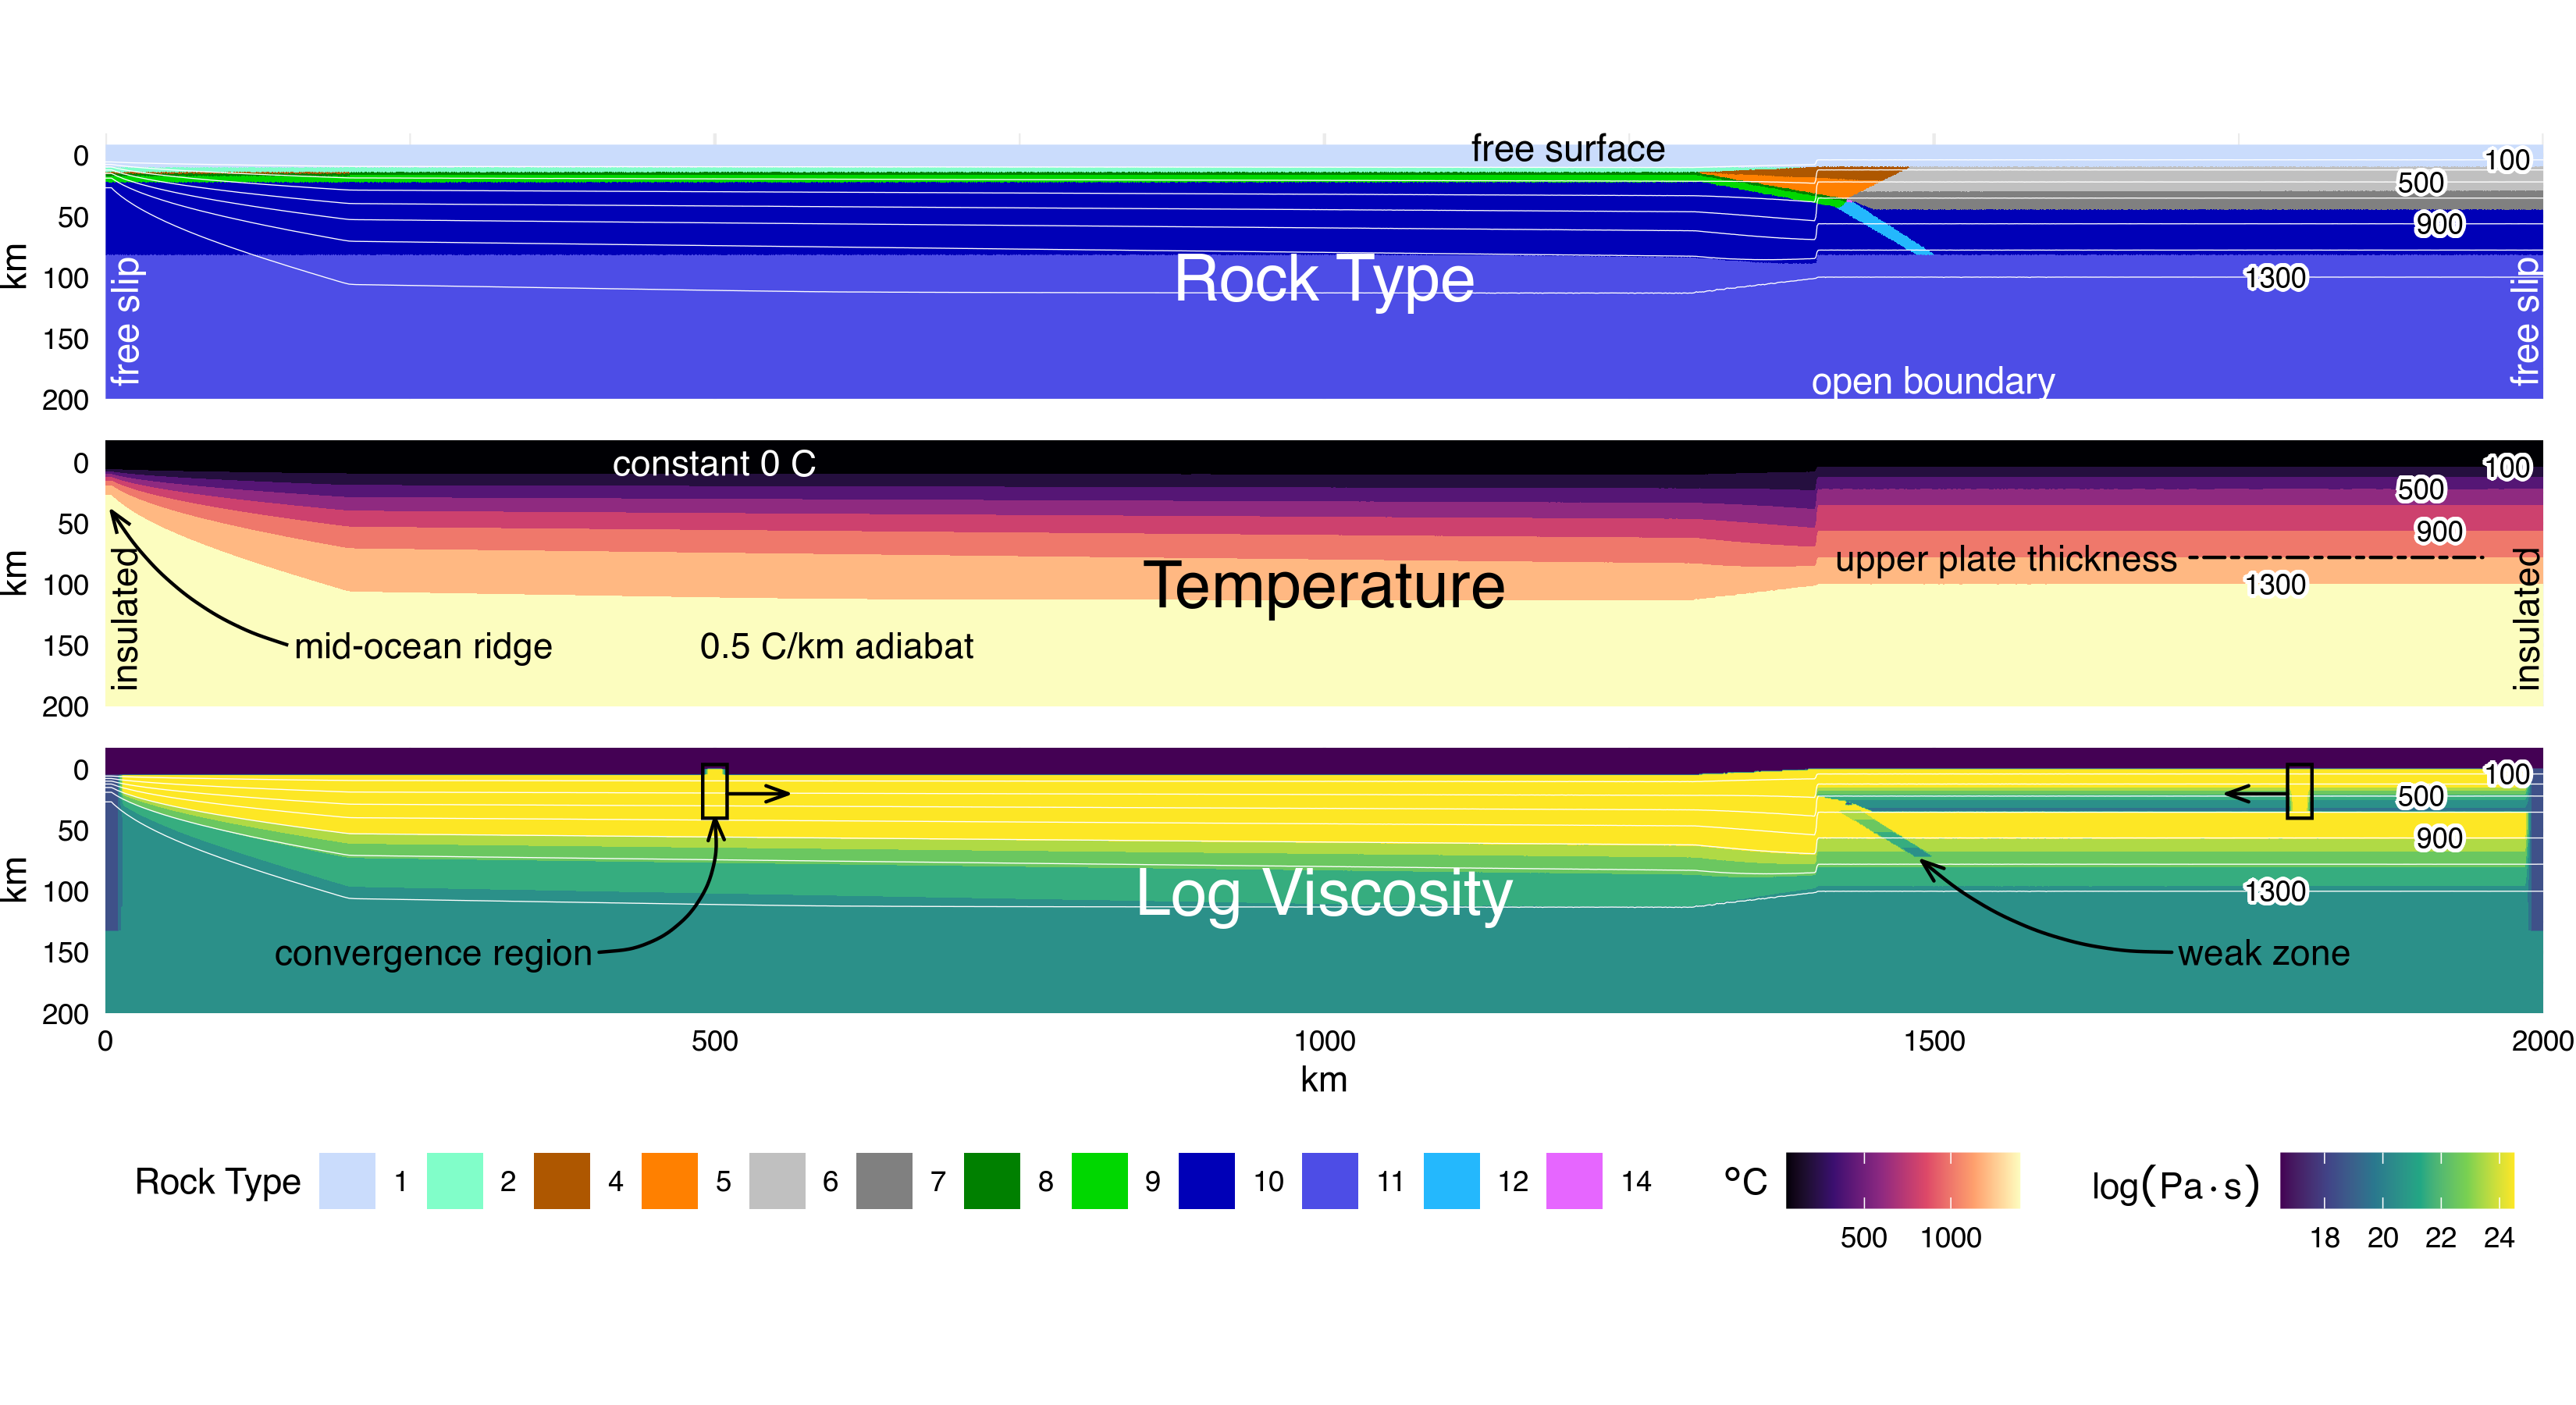
\includegraphics[width=1\linewidth,]{assets/figs/chpt2/fig1} 

}

\caption[Initial model configuration and boundary conditions]{Initial model configuration and boundary conditions. (a) A free sedimentation/erosion boundary at the surface is maintained by implementing a layer of "sticky" air and water, and an infinite-like open boundary at the bottom allows for spontaneous oceanic-plate descent and subduction angle. Left and right boundaries are free slip and thermally insulating. Initial material distribution includes 7 $km$ of oceanic crust (2 $km$ basalt, 5 $km$ gabbro), 1 $km$ of oceanic sediments, and 35 $km$ of continental crust, thinning ocean-ward. (b) Oceanic lithosphere is continually created at the left boundary. The oceanic geotherm is calculated using a half-space cooling model and the continental geotherm is calculated using a one-dimensional steady-state conductive cooling model to 1300 $^{\circ}C$. The base of the upper plate lithosphere ($Z_{UP}$) is defined by visualizing viscosity and generally coincides with the 1100 $^{\circ}C$ isotherm. (c) Oceanic crust is bent under loading from passive margin sediments, and a weak zone extends through the lithosphere to help induce subduction. Convergence velocities are imposed at stationary, high-viscosity regions far from the trench. Rock type colors are: [1] air, [2] water, [4,5] sediments, [6,7] felsic crust, [8] basalt, [9] gabbro, [10,11] dry mantle, [12] hydrated mantle, [14] serpentinized mantle.}\label{fig:init}
\end{figure}

\end{landscape}

\hypertarget{numBCs}{%
\subsection{Initial setup and boundary conditions}\label{numBCs}}

Simulations are 2000 \(km\) wide and 300 \(km\) deep (Figure \ref{fig:init}). In the model domain, three governing equations of heat transport, momentum, and continuity are discretized and solved with a conservative finite-difference marker-in-cell approach on a fully staggered grid as outlined in \citet{gerya2003}. Numerical resolution is non-uniform with higher resolution (1 \(km\) x 1 \(km\)) in a 600 \(km\) wide area surrounding the contact between the oceanic-plate and continental margin, then gradually changing to lower resolution towards the model boundaries (5 \(km\) x 1 \(km\), x- and z-directions, respectively). The left and right boundaries are free-slip and thermally insulating (Figure \ref{fig:init}a, b). Implementation of ``sticky'' air and water allows for a free topographical surface with a simple linear sedimentation and erosion model. The lower boundary is open to allow for oceanic-plate descent with a spontaneous subduction angle \citep{burg2005}.

A horizontal convergence force is applied to both plates in a rectangular region far from the continental margin (Figure \ref{fig:init}c). An initial weak layer cutting the lithosphere permits subduction to initiate. The high-viscosity (\(\eta = 10^{25}~Pa\cdot s\)) rectangular convergence regions apply constant horizontal velocities without deforming the lithosphere. Subduction angle is governed by free-motion of the subducting plate. Similarly, subduction velocity varies with time in response to extension or shortening of the overriding plate. \(\Phi\) is thus calculated as the product of the horizontal convergence velocity and the oceanic-plate age \citep[c.f.][]{mckenzie1969}. For convenience and consistency with the literature, this study presents \(\Phi\) in units of \(km\)/100 (Figure \ref{fig:params}a).

\begin{figure}[htbp]

{\centering 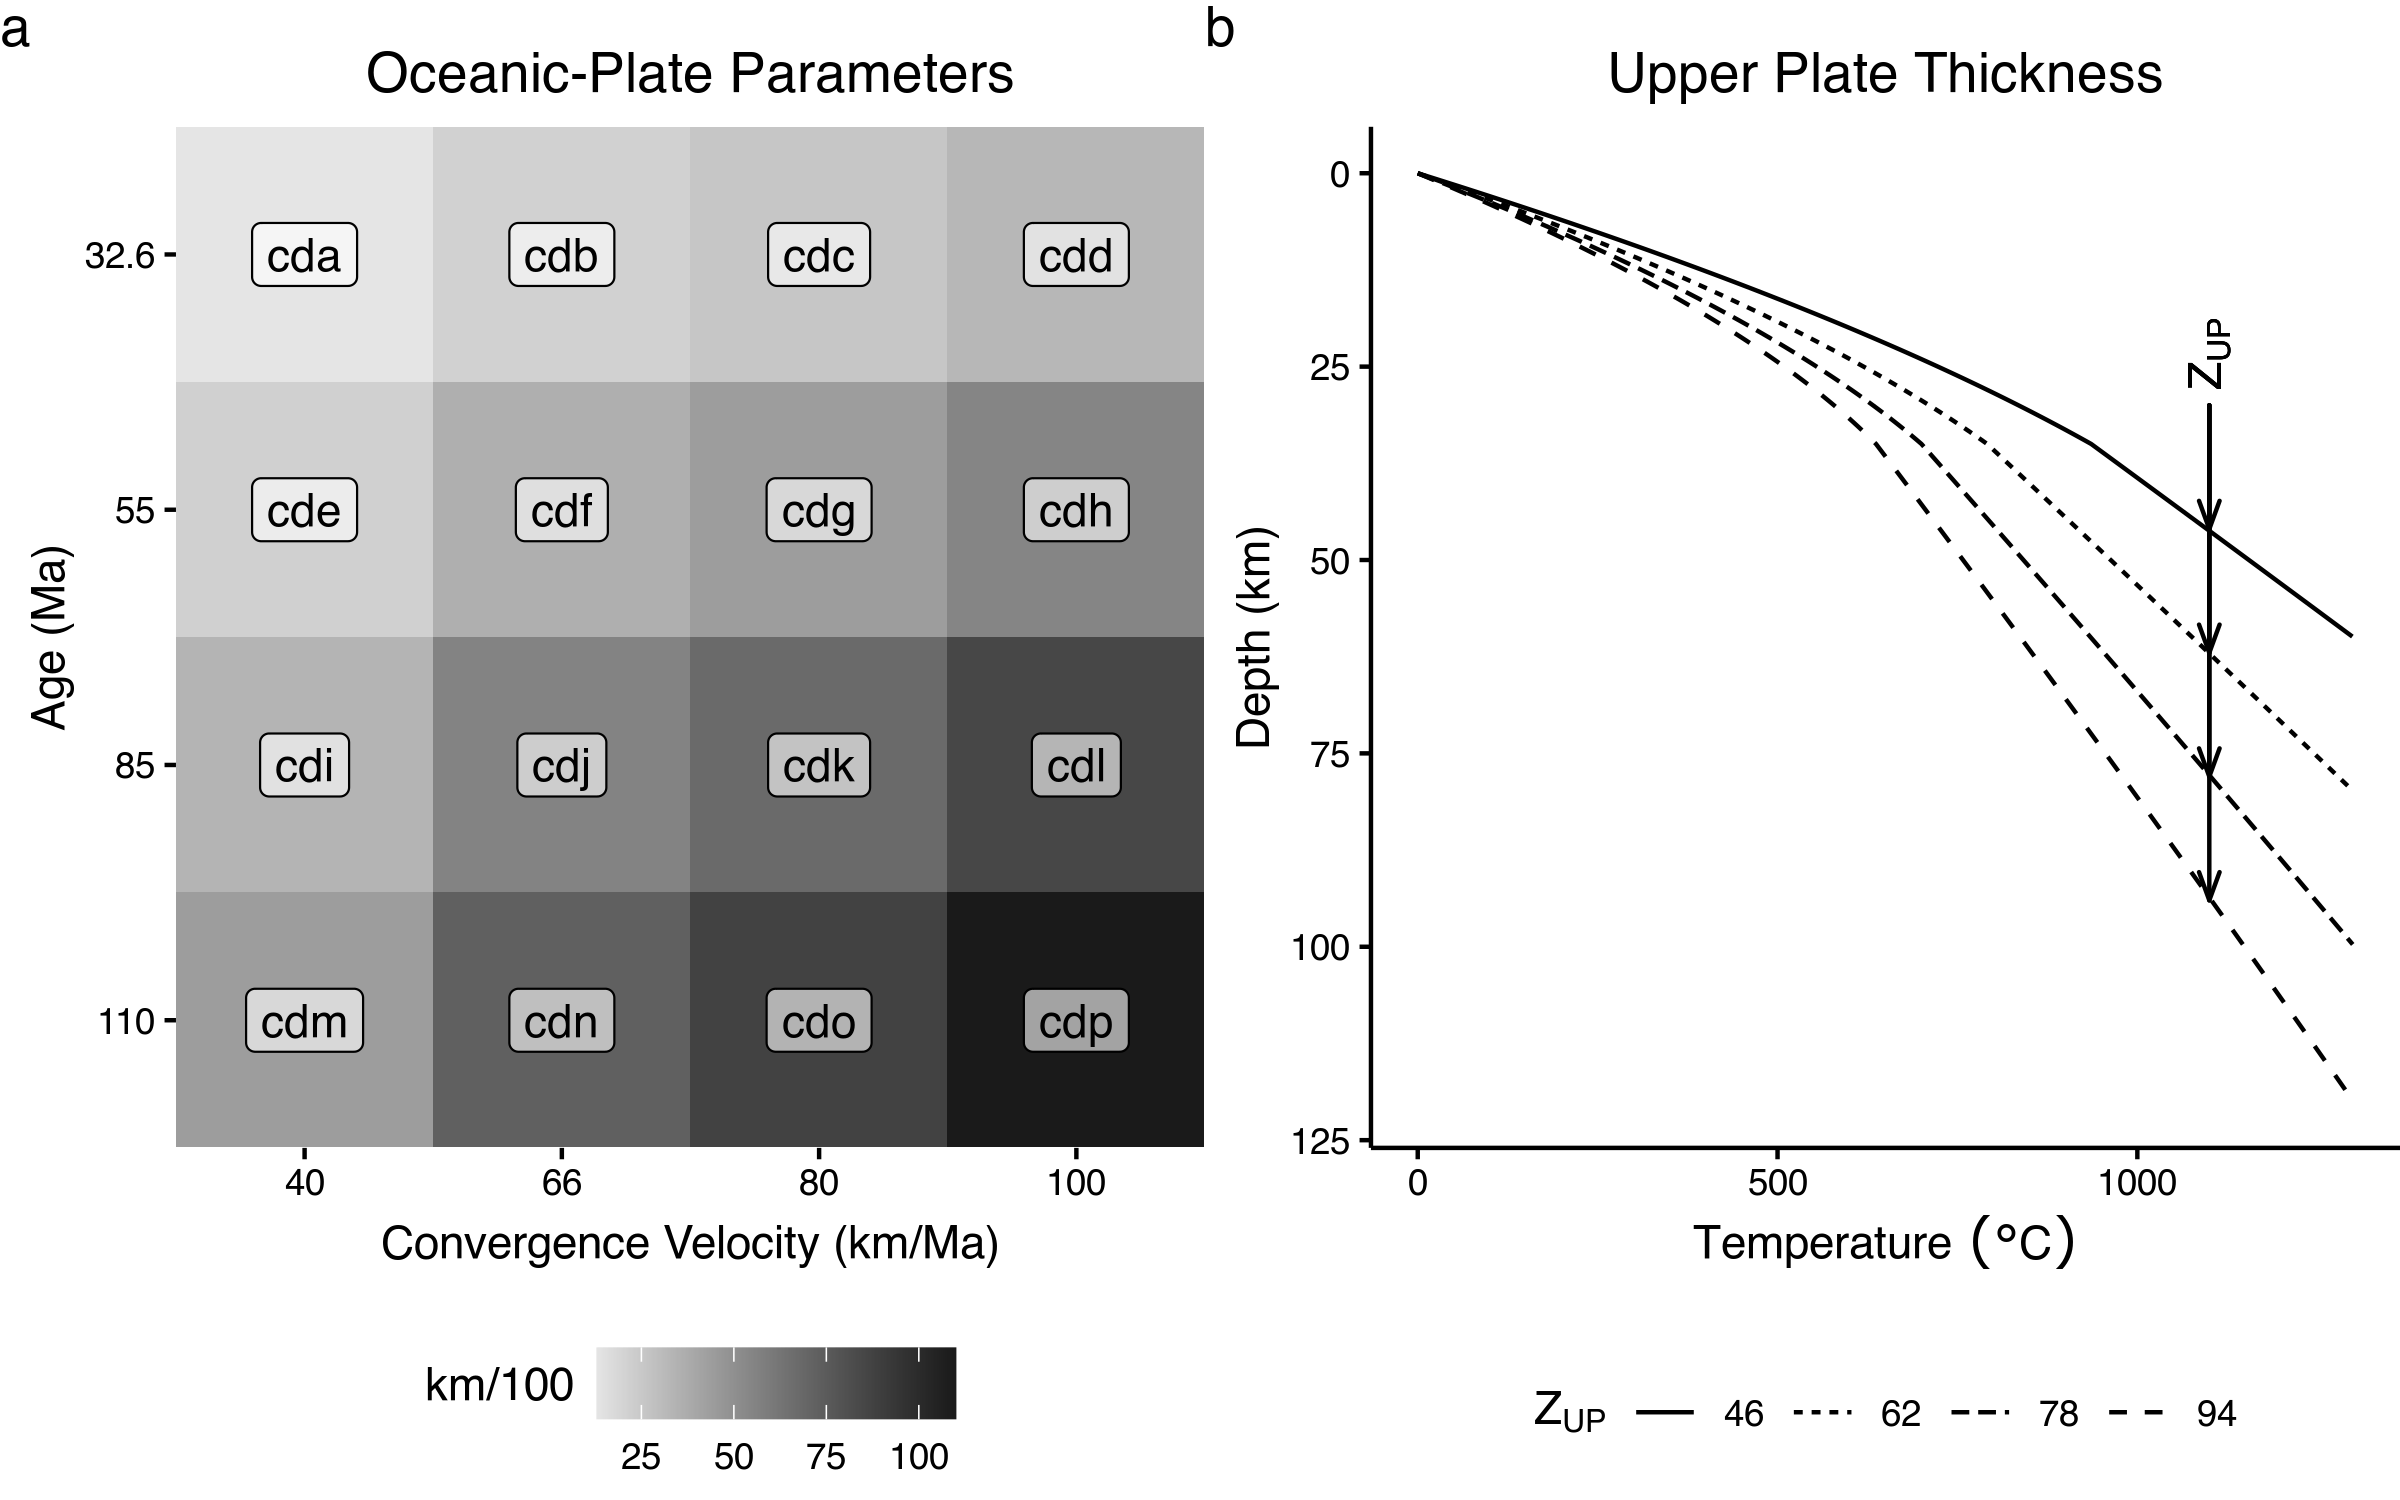
\includegraphics[width=1\linewidth,]{assets/figs/chpt2/fig2} 

}

\caption[Range of thermo-kinematic boundary conditions used in numerical experiments]{Range of thermo-kinematic boundary conditions used in numerical experiments. (a) Thermal parameters (grayscale) range from 13 to 110 $km/100$ and broadly reflect the distribution of oceanic-plate ages and convergence velocities in modern subduction zones. Model names include the prefix "cd" for "coupling depth" with increasing alphabetic suffixes. Note that neither axes are continuous. (b) Upper plate thickness ($Z_{UP}$) is defined by a range of continental geotherms. Geotherms were constructed using a one-dimensional steady-state conductive cooling model with $T(z=0)$ = 0 $^{\circ}C$, $\vec{q}(z=0)$ = 59, 63, 69, 79 $mW/m^2$, and constant radiogenic heating of 1.0 $\mu W/m^3$ for a 35 $km$-thick crust and 0.022 $\mu W/m^3$ for the mantle. Continental geotherms are calculated up to 1300 $^{\circ}$C with a constant 0.5 $^{\circ}C/km$ gradient (the mantle adiabat) extending to the base of the model domain.}\label{fig:params}
\end{figure}

\hypertarget{numGeotherms}{%
\subsection{Calculating geotherms and defining lithospheric thickness}\label{numGeotherms}}

Oceanic crust is modeled as 1 \(km\) of sediment cover overlying 2 \(km\) of basalt and 5 \(km\) of gabbro (Figure \ref{fig:init}a). Oceanic lithosphere is continually made at a pseudo-mid-ocean ridge at the left boundary of the model (Figure \ref{fig:init}b). An enhanced vertical cooling condition applied at 200 \(km\) from left boundary adjusts for the proper oceanic-plate age, and therefore its lithospheric thickness as it enters the trench \citep{agrusta2013}. Oceanic-plate ages range from 32.6 to 110 \(Ma\) and convergence velocities from 40 to 100 \(km/Ma\) (Figure \ref{fig:params}a). This range of parameters broadly reflects the middle-range of modern global subduction systems \citep{syracuse2006}.

Initial continental geotherms are determined by solving the heat flow equation in one-dimension to 1300 \(^{\circ}C\) (Figure \ref{fig:params}b). This study assumes a fixed temperature of 0 \(^{\circ}C\) at the surface, constant radiogenic heating of 1 \(\mu W/m^{3}\) in the 35 \(km\)-thick continental crust, 0.022 \(\mu W/m^{3}\) in the mantle, with thermal conductivities of 2.3 \(W/mK\) and 3.0 \(W/mK\) for the continental crust and mantle, respectively. Above, 1300 \(^{\circ}C\), temperature is assumed to constantly increase by 0.5 \(^{\circ}C/km\) (the mantle adiabat) to the base of the model domain.

Many studies define the base of the continental lithosphere at the 1300 \(^{\circ}C\) isotherm, but it can be determined directly by visualizing viscosity and strain rate as the model progresses. The mechanical base of the lithosphere (\(Z_{UP}\)) in the models generally occurs near the 1100 \(^{\circ}C\) isotherm---characterized by a rapid decrease in viscosity and increase in strain rate (Figures \ref{fig:cdfstep1}, \ref{fig:cdfstep2}, \ref{fig:cdfstep3}). As such, this study considers oceanic and continental lithospheres as mechanical layers defined by viscosity, rather than defined merely by temperature. \(Z_{UP}\) corresponding to backarc surface heat flow of 59, 63, 69, and 79 \(mW/m^{2}\) are used in this study (Figure \ref{fig:params}b).

\hypertarget{numHydration}{%
\subsection{Metamorphic (de)hydration reactions}\label{numHydration}}

Using Lagrangian markers \citep{harlow1962, harlow1964} to store and update material properties and \gls{pts} fields allows for straight-forward numerical implementation of metamorphic reactions. This approach is key to regulating mechanical coupling dynamically in \gls{sz} simulations. For example, dehydration (eclogitization) of the oceanic-plate and (de)stabilization of antigorite in the upper-plate mantle may be effectively modelled by tracing marker \gls{ptt} paths while changing marker properties according to thermodynamically-stable mineral assemblages \citep[e.g.,][]{connolly2005}. For computational efficiency, however, water contents in this study are not computed by iteratively solving thermodynamic systems of equations. Instead, gradual eclogitization of oceanic crust is computed as a linear function of lithostatic pressure to a maximum depth of 150 \(km\), or temperature of 1427 \(^\circ C\), while including garnet-in and plagioclase-out reactions defined by \citet{ito1971}. Mantle (de)hydration is computed according reactions boundaries defined by \citet{schmidt1998} with a maximum water content of 2 \(wt.\%\) (explained below). This approach effectively simulates continuous influx of water to the upper-plate mantle with relatively low computational cost, beginning with compaction and release of connate water at shallow depths, followed by a sequence of reactions consuming major hydrous phases (chlorite, lawsonite, zoisite, chloritoid, talc, amphibole, and phengite) in different parts of the hydrated basaltic crust \citep{schmidt1998, vankeken2011}.

The extent of metamorphic reaction effects on mechanical coupling, and the exact (de)hydration reaction(s) likely responsible, are unknown. However, formation of brucite and serpentine from dry olivine near the plate interface are inferred to strongly regulate mechanical behaviour \citep{hyndman2003, peacock1999a, agard2016}. Brucite notably breaks down at much lower temperatures than serpentine \citep{schmidt1998}, so serpentine (de)stabilization arguably represents the key transition from a weak-to-strong upper-plate mantle deep in \glspl{sz}. This study elects an implement of antigorite (de)hydration for this reason. The reaction is assumed to be abrupt and discontinuous, which is a fine approximation for near-endmember compositions like (Mg-rich) peridotites. The \gls{pt} conditions of the reaction \(antigorite \Leftrightarrow olivine + orthopyroxene + H_{2}O\) were numerically implemented by the following equation \citep[after][]{schmidt1998}:

\begin{equation}
  T_{atg-out}(z)=
  \begin{cases}
    751.50+6.008\times10^{-3}z-3.469\times10^{-8}z^2,& \text{for } z < 63000m \\
    1013.2-6.039\times10^{-5}z-4.289\times10{-9}z^2,& \text{for } z>63000m
  \end{cases}
  \label{eq:antstab}
\end{equation}

where \(z\) is the depth of a marker from the surface in meters and \(T\) is temperature in Kelvins. This reaction boundary is consistent to within 25 \(^{\circ}C\) of more recent experiments by \citet{shen2015}. Markers with internal temperature exceeding \(T_{atg-out}(z)\) spontaneously form \(olivine + orthopyroxene + H_{2}O\) and release their crystal-bound water. This implementation tacitly assumes thermodynamic equilibrium and is common to many versions of \texttt{I2VIS}.

Oceanic-plates of different ages are also tacitly assumed to dehydrate similarly with the above implementation. However, older (colder) oceanic-plates are expected to carry water to greater depths than younger (warmer) plates because of relatively delayed water-releasing reactions \citep{peacock1996}. Abrupt water release at the antigorite dehydration reaction boundary defined by Equation \eqref{eq:antstab} was tested to model deep water retention in cold oceanic-plates. Mechanical coupling behaviour was indistinguishable from gradual water release models. This implies rates of water release are less important than the depth of antigorite dehydration. Explicitly modelling other major dehydration reactions are thus unlikely to significantly affect mechanical coupling behaviour, yet likely to introduce numerical artifacts at great computational cost. A simplified gradual water release model for all oceanic-plates is therefore preferred.

Water released by rock forms discrete fluid particles that migrate with relative velocities defined by local deviatoric (non-lithostatic) pressure gradients \citep[see Appendix @ref(!!!),][]{faccenda2009}. Fluid velocities are scaled by a 10 \(cm/yr\) vertical percolation velocity to account for purely lithostatic pressure gradients in the mantle \citep{gorczyk2007}. Fluid particles migrate until encountering rock that can consume additional water by equilibrium hydration or melting reactions, (Equation \ref{tab:melts}).

The shallow upper-plate mantle can theoretically store large amounts of water as antigorite may contain up to 13 \(wt.\%\) water \citep{reynard2013} and is generally stable at shallow mantle conditions. Thermodynamic models predict 8 \(wt.\%\) water in the shallow upper-plate mantle \citep{connolly2005}. However, seismic studies suggest most shallow upper-plate mantles are only partially serpentinized (\textless{} 20-40\%), equating to water contents of approximately 3-6 \(wt.\%\) \citep{abers2017, carlson2003}. Many modes of mantle hydration are documented or inferred, including evidence for channelized fluid flow within ophiolites exhumed from \glspl{sz} \citep{angiboust2012a, angiboust2014, zack2007, plumper2017}. This study limits mantle wedge hydration to \(\leq\) 2 \(wt.\%~H_{2}O\) and assumes any excess \(H_{2}O\) exits the system through channelized fluid flow during plastic or brittle deformation \citep{davies1999}.

\begin{table}

\caption{\label{tab:materials}Material properties used in numerical experiments}
\centering
\resizebox{\linewidth}{!}{
\begin{threeparttable}
\begin{tabular}[t]{lrrlrrrrrrrrlr}
\toprule
Material & $\rho$ & $H_2O$ & Flow Law & $log_{10}A$ & $E$ & $V$ & $n$ & $\phi$ & $\sigma_{crit}$ & $k_1$ & $k_2$ & $k_3$ & $H$\\
\midrule
\cellcolor{gray!6}{sediments} & \cellcolor{gray!6}{2600} & \cellcolor{gray!6}{5.0} & \cellcolor{gray!6}{wet quartzite} & \cellcolor{gray!6}{-3.5} & \cellcolor{gray!6}{154.0} & \cellcolor{gray!6}{3.0} & \cellcolor{gray!6}{2.3} & \cellcolor{gray!6}{0.15} & \cellcolor{gray!6}{0.03} & \cellcolor{gray!6}{0.64} & \cellcolor{gray!6}{807} & \cellcolor{gray!6}{4e-06} & \cellcolor{gray!6}{2.000}\\
felsic crust & 2700 &  & wet quartzite & -3.5 & 154.0 & 3.0 & 2.3 & 0.45 & 0.03 & 0.64 & 807 & 4e-06 & 1.000\\
\cellcolor{gray!6}{basalt} & \cellcolor{gray!6}{3000} & \cellcolor{gray!6}{5.0} & \cellcolor{gray!6}{plag an75} & \cellcolor{gray!6}{-3.5} & \cellcolor{gray!6}{238.0} & \cellcolor{gray!6}{8.0} & \cellcolor{gray!6}{3.2} & \cellcolor{gray!6}{0.45} & \cellcolor{gray!6}{0.03} & \cellcolor{gray!6}{1.18} & \cellcolor{gray!6}{474} & \cellcolor{gray!6}{4e-06} & \cellcolor{gray!6}{0.250}\\
gabbro & 3000 &  & plag an75 & -3.5 & 238.0 & 8.0 & 3.2 & 0.45 & 0.03 & 1.18 & 474 & 4e-06 & 0.250\\
\cellcolor{gray!6}{mantle dry} & \cellcolor{gray!6}{3300} & \cellcolor{gray!6}{} & \cellcolor{gray!6}{dry olivine} & \cellcolor{gray!6}{4.4} & \cellcolor{gray!6}{540.0} & \cellcolor{gray!6}{20.0} & \cellcolor{gray!6}{3.5} & \cellcolor{gray!6}{0.45} & \cellcolor{gray!6}{0.30} & \cellcolor{gray!6}{0.73} & \cellcolor{gray!6}{1293} & \cellcolor{gray!6}{4e-06} & \cellcolor{gray!6}{0.022}\\
\addlinespace
mantle hydrated & 3300 & 0.5 & wet olivine & 3.3 & 430.0 & 10.0 & 3.0 & 0.45 & 0.24 & 0.73 & 1293 & 4e-06 & 0.022\\
\cellcolor{gray!6}{serpentine} & \cellcolor{gray!6}{3200} & \cellcolor{gray!6}{2.0} & \cellcolor{gray!6}{serpentine} & \cellcolor{gray!6}{3.3} & \cellcolor{gray!6}{8.9} & \cellcolor{gray!6}{3.2} & \cellcolor{gray!6}{3.8} & \cellcolor{gray!6}{0.15} & \cellcolor{gray!6}{3.00} & \cellcolor{gray!6}{0.73} & \cellcolor{gray!6}{1293} & \cellcolor{gray!6}{4e-06} & \cellcolor{gray!6}{0.022}\\
\bottomrule
\end{tabular}
\begin{tablenotes}
\item \uline{\textit{key}}: $\rho$: density $[kg/m^3]$, $H_2O$: water content $[wt.\%]$, $A$: material constant, $E$: activation energy $[kJ/mol]$, $V$: activation volume $[J/MPa\cdot mol]$, $n$: power law exponent, $\phi$: internal friction angle, $\sigma_{crit}$: critical stress $[MPa]$, $H$: heat production $[\mu W/m^3]$
\item \uline{\textit{constants}}: $C_p$: heat capacity = $1~[kJ/kg]$, $\alpha$: expansivity = $2\times 10^{-5}~[1/K]$, $\beta$: compressibility = $0.045~[1/MPa]$
\item \uline{\textit{thermal conductivity}}: $k$ $[W/m \cdot K]=(k_1+\frac{k_2}{T+77})\times exp(k_3 \cdot P)$ with $P$ in $[MPa]$ and $T$ in $[K]$
\item \uline{\textit{references}}: Turcotte \& Schubert (2002), Ranalli (1995), Hilairet et al. (2007), Karato \& Wu (1993)
\end{tablenotes}
\end{threeparttable}}
\end{table}

\hypertarget{rheologic-model}{%
\subsection{Rheologic model}\label{rheologic-model}}

Contributions from dislocation and diffusion creep are accounted for by computing a composite rheology for ductile rocks, \(\eta_{effective}\):

\begin{equation}
  \begin{aligned}
    \frac{1}{\eta_{effective}} = \frac{1}{\eta_{diff}} + \frac{1}{\eta_{disl}}
  \end{aligned} 
  \label{eq:ductile}
\end{equation}

where \(\eta_{diff}\) and \(\eta_{disl}\) are effective viscosities for diffusion and dislocation creep.

For the crust and serpentinized mantle, \(\eta_{diff}\) and \(\eta_{disl}\) are computed as:

\begin{equation}
  \begin{aligned}
    \eta_{diff} &= \frac{1}{2} \ A \ \sigma_{crit}^{1-n} \ \exp\left[\frac{E+PV}{RT}\right] \\
    \eta_{disl} &= \frac{1}{2} \ A^{1/n} \ \dot{\varepsilon}_{II}^{(1-n)/n} \ \exp\left[\frac{E+PV}{nRT}\right]
  \label{eq:crust}
  \end{aligned}
\end{equation}

where \(R\) is the gas constant, \(P\) is pressure, \(T\) is temperature in \(K\), \({\dot{\varepsilon}}_{II} = \sqrt{\frac{1}{2}{{\dot{\varepsilon}}_{ij}}^{2}}\) is the square root of the second invariant of the strain rate tensor, \(\sigma_{crit}\) is an assumed diffusion-dislocation transition stress, and \(A\), \(E\), \(V\) and \(n\) are the material constant, activation energy, activation volume, and stress exponent, respectively \citep[Table \ref{tab:materials},][]{Hilairet2007, Ranalli1995}.

For the mantle, \(\eta_{diff}\) and \(\eta_{disl}\) are computed as \citep{Karato1993}:

\begin{equation}
  \begin{aligned}
    \eta_{diff} &= \frac{1}{2} \ A^{-1} \ G \ \left[\frac{h}{b}\right]^{m/n} \ \exp\left[\frac{E+PV}{RT}\right] \\
    \eta_{disl} &= \frac{1}{2} \ A^{-1/n} \ G \ \dot{\varepsilon}_{II}^{(1-n)/n} \ \exp\left[\frac{E+PV}{nRT}\right]
  \end{aligned}
  \label{eq:mantle}
\end{equation}

where \(b\)=\(5\times10^{-10}\) \(m\) is Burgers vector, \(G\)=\(8\times10^{10}\) \(Pa\) is shear modulus, \(h\)=\(1\times10^{-3}\) \(m\) is the assumed grain size, \(m=2.5\) is the grain size exponent, and the other flow law parameters are given in Table \ref{tab:materials}. Our models limited viscosity for all rocks at \(\eta_{min} = 10^{17}\ Pa \cdot s\) and \(\eta_{max} = 10^{25}\ Pa \cdot s\).

An effective visco-plastic rheology is achieved by limiting \(\eta_{effective}\) with a brittle (plastic) yield criterion:

\begin{equation}
  \eta_{effective} \leq \frac{C + \phi \ P}{2 \ \dot{\varepsilon}_{II}}
  \label{eq:plastic}
\end{equation}

\hypertarget{visualization-and-determination-of-coupling-depth}{%
\subsection{Visualization and determination of coupling depth}\label{visualization-and-determination-of-coupling-depth}}

The rheologic model and \gls{tkbc} described in the previous sections always results in plate motions towards the left boundary (slab-rollback). Relatively high dip angles and extreme subduction velocities in the some high-\(\Phi\) experiments cause chaotic behaviour by 10 \(Ma\) as the upper-plate is stretched thin and mechanical interference occurs between trench sediments and the high-viscosity convergence region 200 \(km\) from the left boundary. Numerical solutions are stable for most experiments, however, reaching quasi-steady state by 5 \(Ma\). An additional 5 \(Ma\) is allowed to ensure stable geodynamics before observing \gls{cd}. Surface heat flow, rock type, temperature, viscosity, strain rate, shear heating, and velocity fields are visualized at approximately 10 \(Ma\) (e.g., Figure \ref{fig:comp}) for all 64 experiments to assess geodynamics and solution stability (Figure \ref{fig:antdepth}).

After approximately 10 \(Ma\) of subduction \gls{cd} is determined directly from viscosity by finding the approximate area where strength contrasts between serpentinized- and non-serpentinized upper-plate mantle diminishes to \(<\) 10\(^{2}\) \(Pa \cdot s\). The node nearest to this region is assigned as the \gls{cd}. This study assumes mechanical coupling occurs instantaneously and at a single node. Mechanical coupling in reality must be dispersed across a finite length along the plate interface, however. At the numerical resolution the experiments, coupling-like viscosity contrasts are similar within a small area (approximately 5x5 \(km\) or 5x5 nodes), giving a qualitative uncertainty \gls{cd} on the order of 2.5 \(km\).

\begin{figure}[htbp]

{\centering \includegraphics[width=1\linewidth,]{assets/figs/chpt2/fig3_notitle} 

}

\caption[Visualization of rock type, viscosity, stream lines, and strain rate for model cdf]{Visualization of model cdf with a 78 $km$ upper-plate lithosphere at approximately 10 $Ma$. (a) Rock type shows a thin serpentine layer (pink) lubricating the plate interface. Note that low melt volumes are inconspicuous and quickly extracted. (b) Viscosity shows high contrast between the oceanic-plate and serpentinized upper-plate mantle at shallow levels. Viscosity contrast disappears where serpentine becomes unstable. (c) Streamlines show focused mantle flow towards the interface, coinciding with the lower limit of serpentine stability. Note the converging isotherms that imply a feedback between heat transfer, serpentine destabilization, and mechanical coupling. (d) Strain rate shows localized deformation in the serpentine layer along the plate interface. Note that deformation in the upper-plate mantle is restricted to viscous flow beneath the lithosphere and along narrow, subvertical melt conduits. Rock type colors are the same as Figure 1.}\label{fig:comp}
\end{figure}

\cleardoublepage

\hypertarget{chpt3}{%
\chapter{A Comparison of Heat Flow Interpolations Near Subduction Zones}\label{chpt3}}

\markboth{Chapter 3: Heat Flow Interpolations}{Chapter 2: Heat Flow Interpolations}

\begin{quote}
\textbf{Keypoints:}

\begin{itemize}
\item
  Inconsistent spatial patterns characterize heat flow near subduction zones
\item
  Heat flow investigations favour 2D interpolations over 1D transects
\item
  Scaling datasets and new interpolation schema will advance \gls{sz} research
\end{itemize}
\end{quote}

\hypertarget{abstract-1}{%
\section{Abstract}\label{abstract-1}}

Heat fluxing through the Earth's surface provides indirect observations of \glsfirst{pts} fields deep in \glspl{sz}. Global heat flow databases, therefore, are invaluable for generating and testing belief about \gls{sz} geodynamics. Investigating \glsfirst{shf} in two-dimensions by interpolation, rather than in one-dimension by projection, arguably forms better interpretations about spatial continuity of deep processes. Direct comparisons of interpolations based on the First (spatial continuity) and Third (similarity) Laws of Geography applied to the most updated global heat flow database. Inconsistent spatial patterns of \gls{shf} near \glspl{sz} are observed in magnitude and variance, regardless of interpolation method. The implications include discontinuous \gls{pts} fields at depth, countering hypotheses of commonly thin upper plate lithospheres and mechanical \glspl{cd} among subduction zones. Strategic scaling of \gls{shf} datasets will improve interpolation precision and confidence---leading to better tools for distinguishing differences within and among \glspl{sz}. New data acquisition and composite interpolation schema are proposed as avenues for future \gls{sz} research.

\cleardoublepage

\hypertarget{refs}{}
\begin{CSLReferences}{0}{0}
\end{CSLReferences}

\markboth{References}{References}

\hypertarget{appendix-appendix}{%
\appendix}


\hypertarget{section}{%
\chapter{}\label{section}}

\hypertarget{deHydration}{%
\section{(De-)hydration model}\label{deHydration}}

The material properties used in our experiments are listed in Table \ref{tab:materials} and Table \ref{tab:melts}. For details about the sedimentation and erosion, melting and extraction, and rheological models, please refer to \citet{sizova2010}. Here we discuss only the hydrodynamic model, because it is the most relevant aspect of our results.

The hydrodynamics in our models controls the timing and magnitude of mantle wedge hydration. The main sources of water delivered to the mantle are altered basaltic crust and seafloor sediments, which we assumed to contain up to 5 \(wt.\% H_{2}O\). We assumed a gradual expulsion of water from pore space and through quasi-continuous dehydration reactions occurring within the slab. Water content is computed using the following equation:

\begin{equation}
  \begin{aligned}
    \chi_{H_{2}O(wt.\%)} = \chi_{H_{2}O(p_{0})} \times \left( 1 - \frac{\Delta z}{150 \cdot 10^{3}} \right)
  \end{aligned}
\end{equation}

where \(\chi_{H_{2}O(p_{0})}\)=5 \(wt.\%\) and \(\Delta z\) is a marker's depth below the topographical surface.

If a rock marker dehydrates, an independent water particle is instantaneously generated at the same location with the respective \(H_{2}O\) content. The new water particle is moved in accordance to the local velocity field, described by the following equation:

\begin{equation}
  \begin{aligned}
    v_{\text{water}} & = (v_{x(\text{fluid})},v_{z(\text{fluid})}) \\
    v_{z(\text{fluid})} & = v_{z(\text{fluid})} - v_{z(\text{percolation})} \\
  \end{aligned}
\end{equation}

where \(v_{water}\) is the velocity vector of the water particle, \(v_{x}\) and \(v_{z}\) are the local velocity vectors of the the solid state mantle or crust, and \(v_{z(percolation)}\) is a prescribed upward percolation velocity (10 \(cm/year\)). We implicitly neglect kinetics of reactions, as material properties of markers change instantaneously at equilibrium reactions.

\begin{table}

\caption{\label{tab:melts}Melting curves used in numerical experiments}
\centering
\resizebox{\linewidth}{!}{
\begin{threeparttable}
\begin{tabular}[t]{lrrlrlrllrr}
\toprule
Material & a & b & c & d & e & f & g & h & i & j\\
\midrule
\cellcolor{gray!6}{sediments} & \cellcolor{gray!6}{1200} & \cellcolor{gray!6}{889} & \cellcolor{gray!6}{1.79e+04} & \cellcolor{gray!6}{54} & \cellcolor{gray!6}{2.02e+04} & \cellcolor{gray!6}{831} & \cellcolor{gray!6}{6.00e-02} & \cellcolor{gray!6}{} & \cellcolor{gray!6}{1262} & \cellcolor{gray!6}{0.009}\\
felsic crust & 1200 & 889 & 1.79e+04 & 54 & 2.02e+04 & 831 & 6.00e-02 &  & 1262 & 0.009\\
\cellcolor{gray!6}{basalt} & \cellcolor{gray!6}{1600} & \cellcolor{gray!6}{973} & \cellcolor{gray!6}{7.04e+05} & \cellcolor{gray!6}{354} & \cellcolor{gray!6}{7.78e+07} & \cellcolor{gray!6}{935} & \cellcolor{gray!6}{3.50e-03} & \cellcolor{gray!6}{6.2e-05} & \cellcolor{gray!6}{1423} & \cellcolor{gray!6}{0.105}\\
gabbro & 1600 & 973 & 7.04e+05 & 354 & 7.78e+07 & 935 & 3.50e-03 & 6.2e-05 & 1423 & 0.105\\
\cellcolor{gray!6}{mantle dry} & \cellcolor{gray!6}{} & \cellcolor{gray!6}{} & \cellcolor{gray!6}{} & \cellcolor{gray!6}{} & \cellcolor{gray!6}{} & \cellcolor{gray!6}{1394} & \cellcolor{gray!6}{1.33e-01} & \cellcolor{gray!6}{-5.1e-05} & \cellcolor{gray!6}{2073} & \cellcolor{gray!6}{0.114}\\
\addlinespace
mantle hydrated & 2400 & 1240 & 4.98e+04 & 323 &  &  & 1.27e+05 & 3.5e-05 & 2073 & 0.114\\
\cellcolor{gray!6}{serpentine} & \cellcolor{gray!6}{2400} & \cellcolor{gray!6}{1240} & \cellcolor{gray!6}{4.98e+04} & \cellcolor{gray!6}{323} & \cellcolor{gray!6}{} & \cellcolor{gray!6}{} & \cellcolor{gray!6}{1.27e+05} & \cellcolor{gray!6}{3.5e-05} & \cellcolor{gray!6}{2073} & \cellcolor{gray!6}{0.114}\\
\bottomrule
\end{tabular}
\begin{tablenotes}
\item \uline{\textit{solidus curve}}: $T(P)=[b+\frac{c}{(P+d)}+\frac{e}{(P+d)^2}]$ at $P<a$ and $[f+gP+hP^2]$ at $P\geq a$
\item \uline{\textit{liquidus curve}}: $T(P) = i+jP$ with $T$ in $[K]$ and $P$ in $[MPa]$
\item \uline{\textit{reference}}: Schmidt \& Poli (1998)
\end{tablenotes}
\end{threeparttable}}
\end{table}

% Bibliography
\renewcommand\bibname{REFERENCES}
\phantomsection
\cleardoublepage
\addcontentsline{toc}{chapter}{References}
\bibliography{assets/bib/chpt2/ref.bib}

\end{document}
